\documentclass[a4paper,12pt]{article}
\usepackage{color}
\usepackage{url}
\usepackage{graphicx}
\usepackage{amsmath}
\usepackage{caption}
\usepackage{subcaption}
\usepackage[font=footnotesize]{caption}
\graphicspath{ {./images/} }

\setlength{\oddsidemargin}{0mm}
\setlength{\evensidemargin}{-14mm}
\setlength{\marginparwidth}{0cm}
\setlength{\marginparsep}{0cm}
\setlength{\topmargin}{2mm}
\setlength{\headheight}{0mm}
\setlength{\headsep}{0cm}
\setlength{\textheight}{240mm}
\setlength{\textwidth}{168mm}
\setlength{\topskip}{0mm}
\setlength{\footskip}{10mm}
\setlength{\parindent}{8ex}

\newcommand{\comment}[1]{\emph{\color{blue}#1}}


\title{ENMT482 Assignment 1}
\author{Oliver Dale and Josh Roberts, Group 18}
\date{}

\begin{document}
\maketitle

\section{Sensor fusion}


\subsection{Sensor models}
A linear model, $h(x)=cx+d$ and a hyperbolic model, $h(x)=c/x+d$, were used to create the sensor models for the sonar and IR sensors respectively. Outliers were removed from the sensor readings by iteratively removing the points furthest from the line of best fit. The error at each data point was found, $v(x)=z-h(x)$, then passed through a MAF with window size 50 which calculated the standard deviation within each window. A polynomial was fitted to give the standard deviation as a function of displacement. The calibration plots, sensor models, and standard deviation models for the three sensors used are included in the Appendix. Sonar 1, IR 1, and IR 4 were chosen as they worked over the widest range and produced more consistent results.
 

\subsection{Motion model}
An improved motion model (1) was created by using a better estimate of the velocity $\hat{u}_{n-1}$ which was calculated by using the previous velocity estimate $\hat{u}_{n-2}$ as well as the command velocity $u_{n-1}$.

\begin{equation}
g(u_{(n-1)}, x_{(n-1)} )=\hat{u}_{(n-1)}×\Delta t 
\end{equation}

\begin{equation}
        f(r_i)=
        \left\{ \begin{array}{ll}
            u_{n-1} &u_{n-1}=0\\
            \hat{u}_{(n-2)}+0.1×(u_{(n-1)}-\hat{u}_{(n-2)} )+\frac{0.002}{\Delta t} (u_{(n-1)}-\hat{u}_{(n-2)} ) &\text{else}
        \end{array} \right.
	\end{equation}

This model is in the form of a PD controller and prevented the modelled velocity from being able to change instantaneously. The derivative control aims to bring the rate of change of error to zero and greatly improved the variance with a frequently changing velocity command. The estimated, commanded, and modelled velocities for training 1 and training 2 are shown in Fig. 1. The error was determined by finding the difference between the modelled and the true displacement at each time step. The standard deviation of this error array was then calculated. 

With the training 1 and training 2 datasets, our model had a standard deviation 16\% and 47\% lower respectively than the crude model. A fixed standard deviation was used for the motion model by averaging the two standard deviations taken from each training dataset to give $\sigma_{W}=0.1157$.

\begin{figure}[h]
\centering
\begin{subfigure}{.5\textwidth}
  \centering
  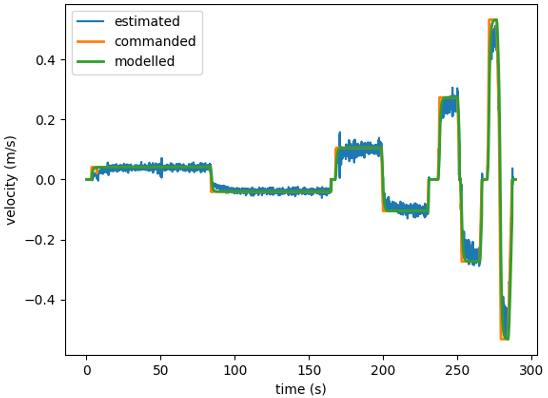
\includegraphics[width=0.9\linewidth]{training1}
\end{subfigure}%
\begin{subfigure}{.5\textwidth}
  \centering
  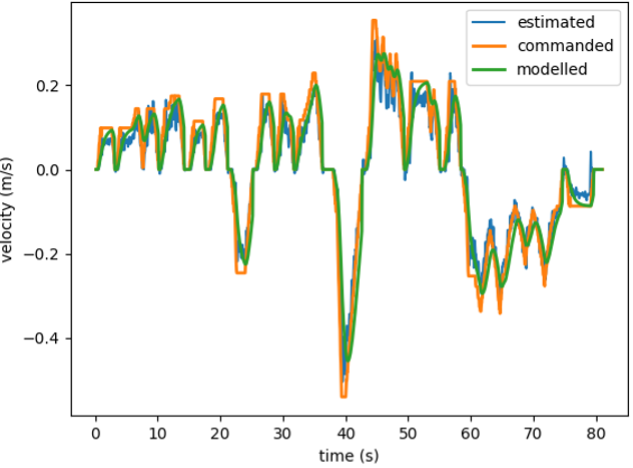
\includegraphics[width=0.9\linewidth]{training2}
\end{subfigure}
\caption{Estimated, commanded, and modelled velocities of the training 1 (left) and 2 (right) data.}
\end{figure}

\subsection{Bayes filter}
An extended Kalman filter (EKF) was used due to the non-linear IR sensor models. A standard Kalman filter is not applicable for non-linear models since the mapping of Gaussian random variable by a non-linear function produces a random variable with a non-Gaussian PDF. Figure 2 shows the functionality of the EKF.

\begin{figure}[h]
\centering
\begin{subfigure}{.5\textwidth}
  \centering
  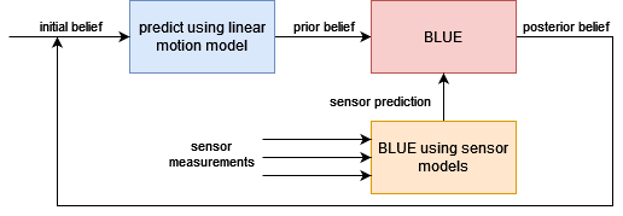
\includegraphics[width=1.1\linewidth]{bayesdiagram}
\end{subfigure}%
\begin{subfigure}{.5\textwidth}
  \centering
  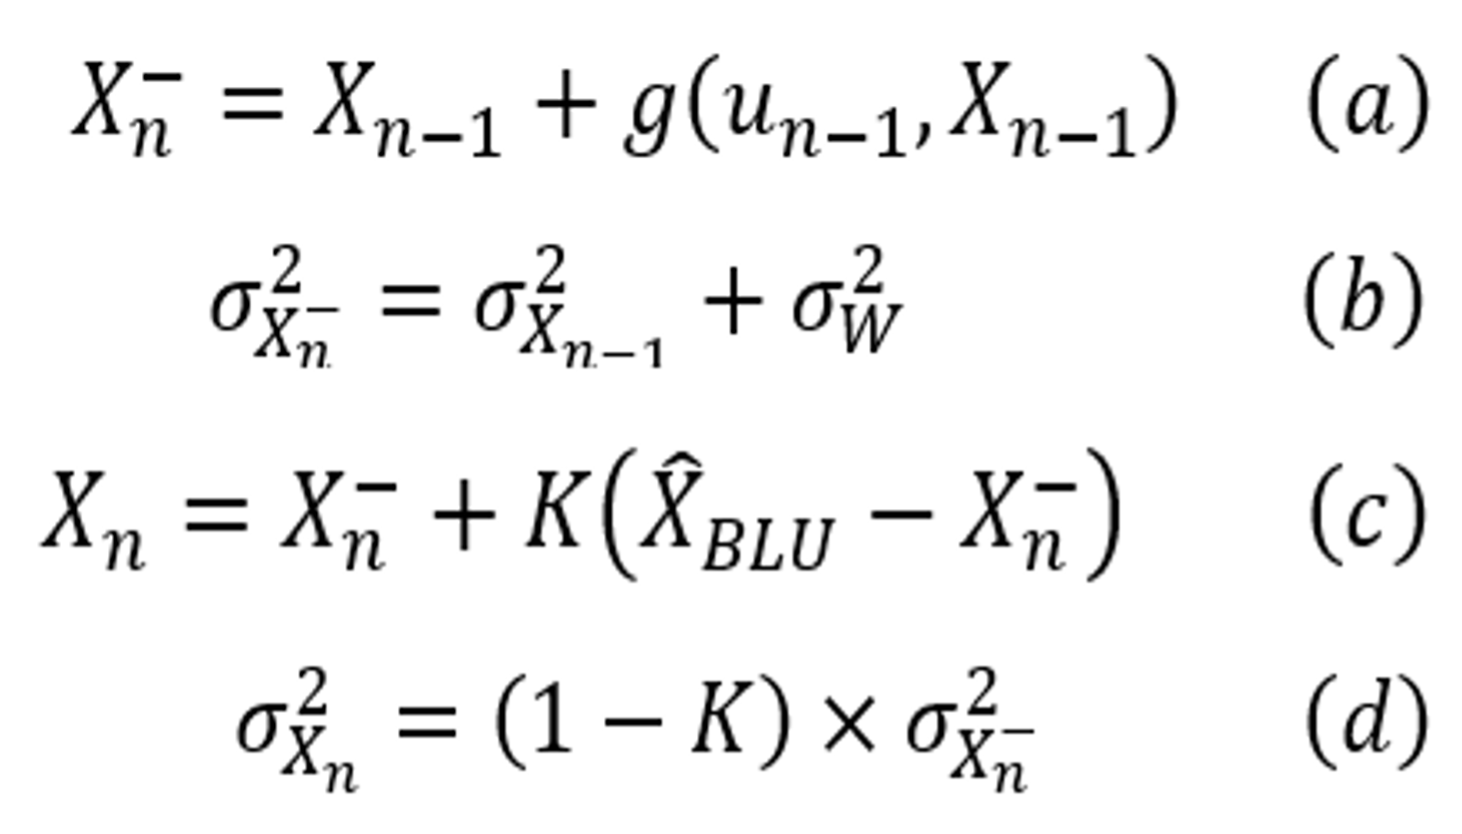
\includegraphics[width=0.6\linewidth]{bayeseq}
\end{subfigure}
\caption{Block diagram of EKF process with equations for prior estimate (a), prior estimate variance (b), posterior estimate (c), and posterior estimate variance (d).}
\end{figure}

\underline{Initialisation:} The starting position of the robot is unknown. A reasonable estimate can be determined by using the first measurement from the sensors. Using a BLUE as described in the update step, the distribution for the initial position of the test dataset was determined as $X_0 \sim \mathcal{N}(0.77644,0.171)$.
\\
\underline{Prediction:} The prediction step determines a prior belief for the displacement of the robot at the current time step given an estimate for the displacement at the previous time step. The prior belief calculation is shown in Figure 2 (a) with corresponding variance (b).
\\
\underline{Update:} The MLE of each sensor measurement is found using the inverse sensor models. In our case, both sensor models are invertible. For the linear sensor model, the variance for the estimate can be calculated directly from the sensor model variance, $\sigma_{\hat{X}}^2(x) = \frac{\sigma_{V}^2(x)}{c^2}$ . For the non-linear IR models, linearisation is required using a Taylor series expansion. This gives a variance for the estimate . The sensor prediction is determined by fusing the three sensor predictions using a BLUE to create a best sensor estimate. This combined sensor prediction is then combined with the prior belief using another BLUE to give a posterior belief shown in Figure 2 (c) with corresponding variance (d).

\subsection{Results}
The output of the Kalman filter is shown for the two training datasets in Figure 3 along with the true position. The standard deviation of the estimate is also plotted.

\begin{figure}[h]
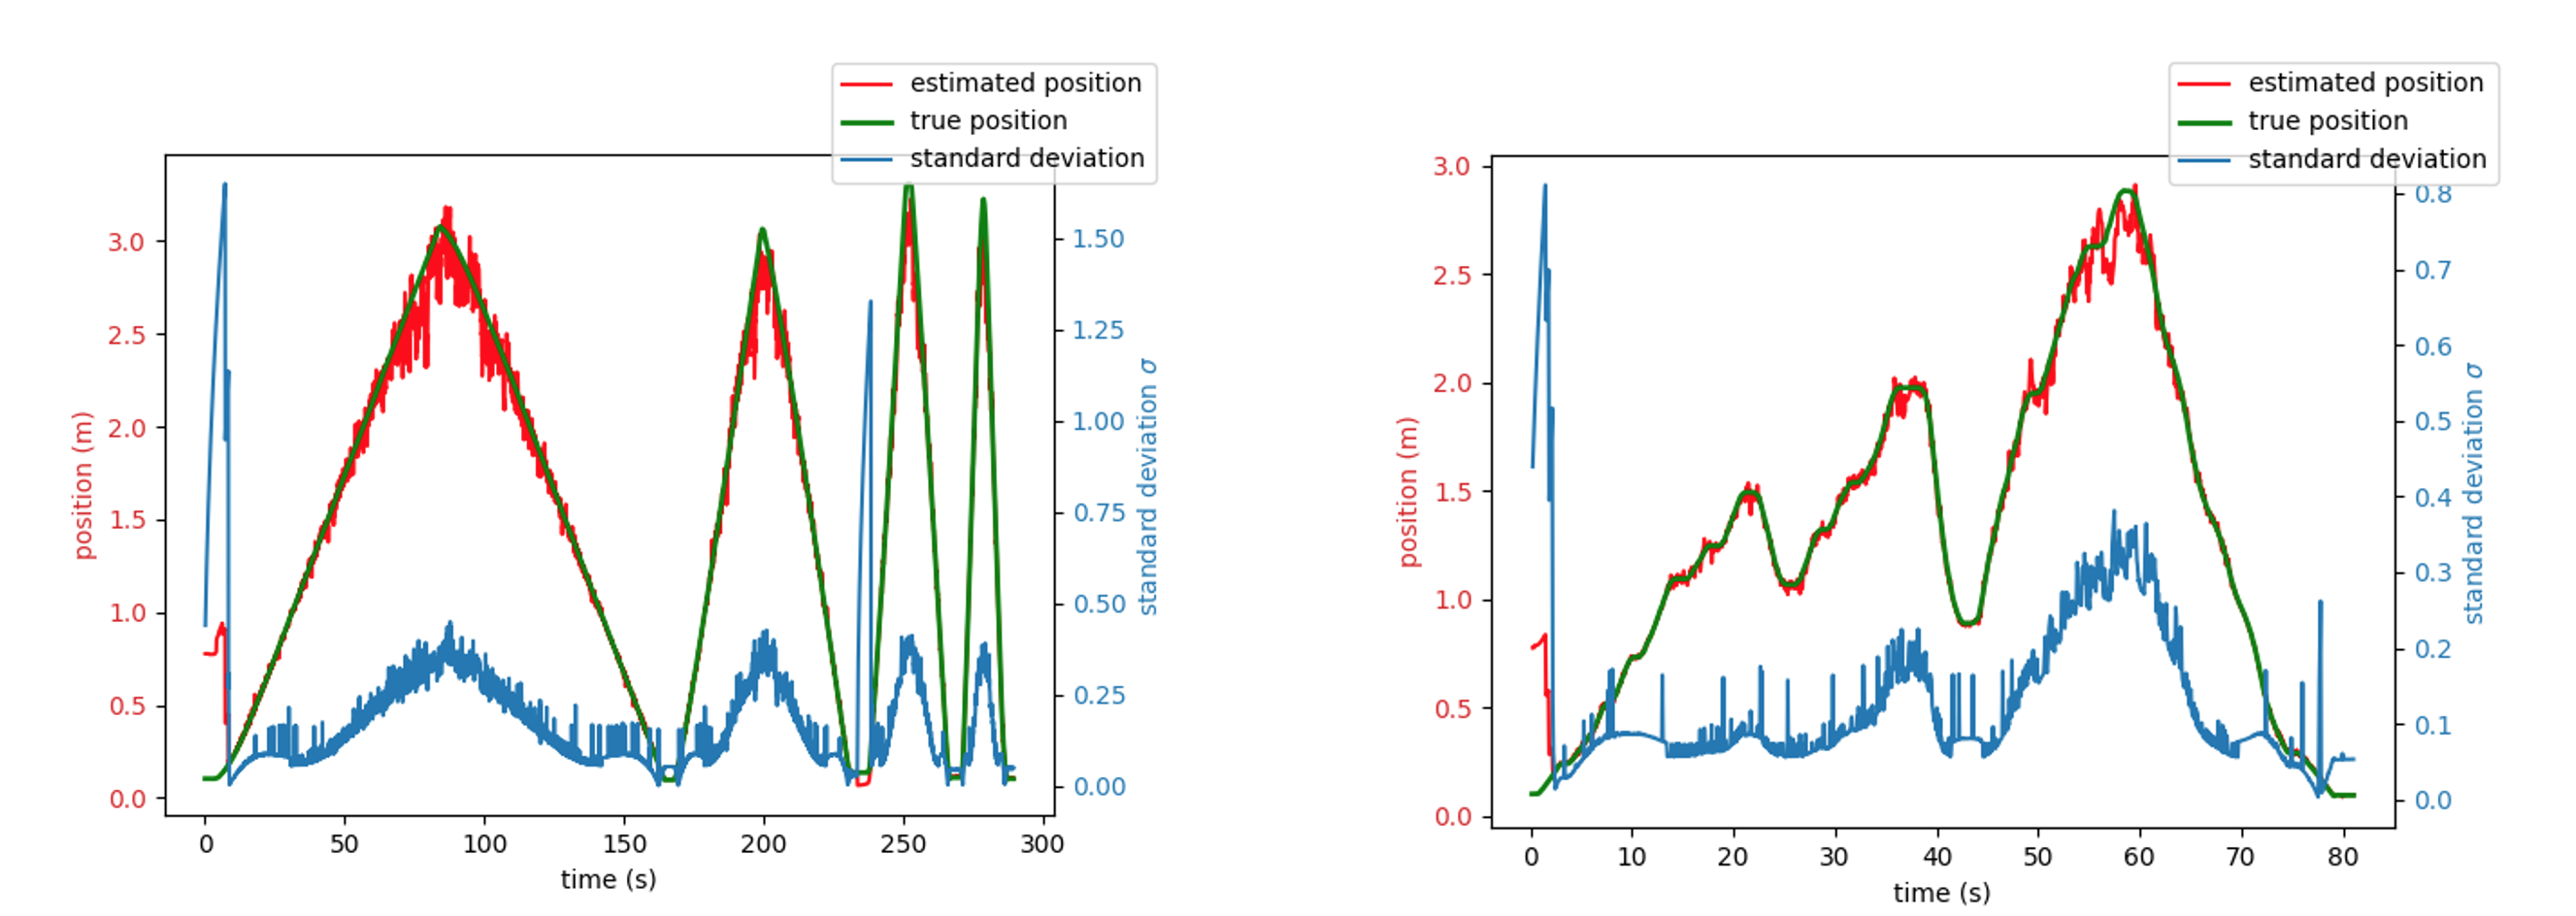
\includegraphics[width=16cm]{result1}
\centering
\caption{Sensor Model}
\end{figure}

Figure 4 shows the output of the Kalman filter with the corresponding standard deviation for the test dataset. Figure 5 shows the corresponding weights.

\begin{figure}[h]
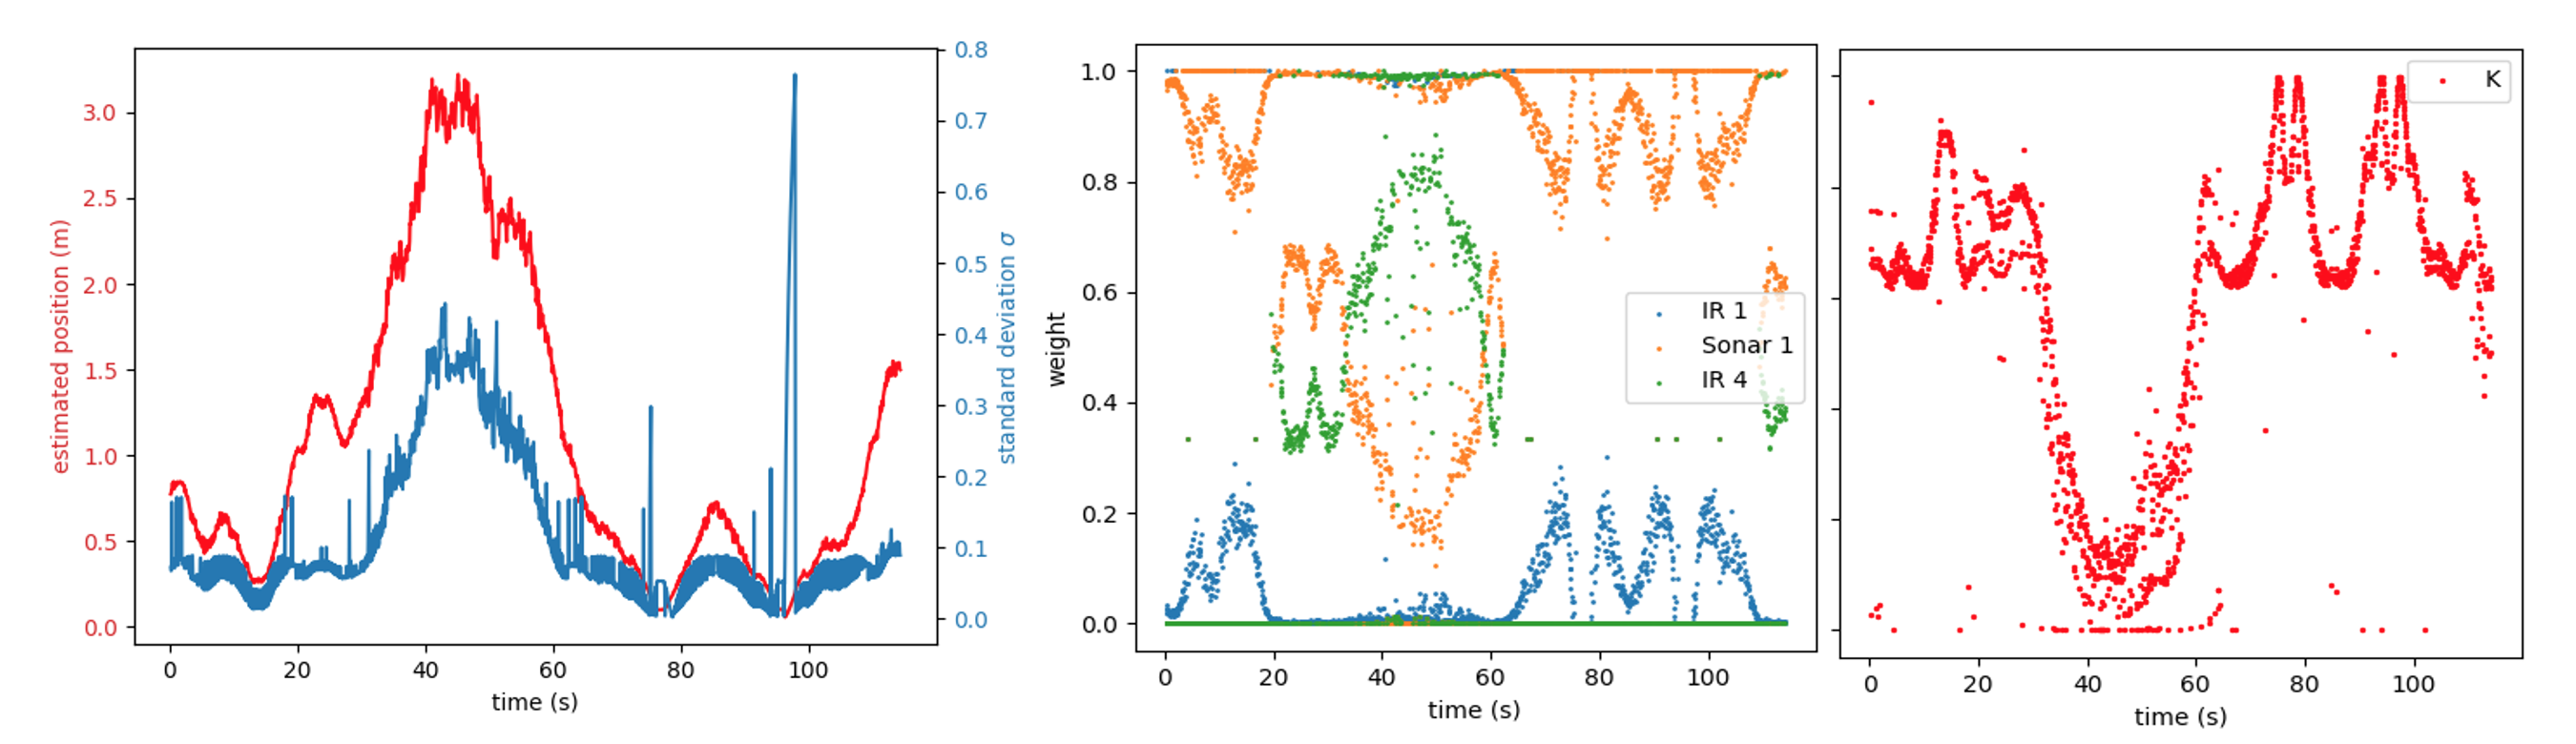
\includegraphics[width=16cm]{results2}
\centering
\caption{Sensor Model}
\end{figure}

\subsection{Discussion}
\underline{Worked well:} The filter accurately tracked the robot location, particularly within a range up to 1.5 m. Beyond this, the filter output was much noisier, reflecting the higher variances of the sensors at a larger range. The filter was able to successfully locate the robot given an inaccurate starting position as shown in Figure 3. This shows that the filter does not rely too heavily on the motion model. Sensor outliers are successfully accounted for by rejecting sensor position estimates that fall more than one standard deviation away from the prior estimate. These measurements have a 68.2\% probability of being outliers.
\\
\underline{Improvements:} The filter could be improved using an unscented Kalman filter (UKF). A UKF can produce a better approximation of a Gaussian distribution from a non-linear function by computing a set of sigma points. The noise could be improved by adding a sensor with a low variance at higher ranges. 



\section{Particle filter}

\subsection{Sensor model}

The sensor model updated the particle weights based on the beacon measurements (Fig. X).

\begin{figure}[h]
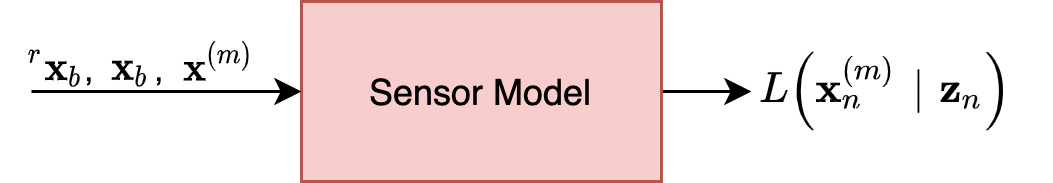
\includegraphics[width=8cm]{PartBSensor}
\centering
\caption{Sensor Model}
\end{figure}

The beacon pose was converted to a range and bearing to decouple the likelihood function. Each particle calculated its corresponding range and bearing to the beacons global location, which were compared with the measured beacon pose. The particles were then weighted on how close their calculated range and bearing matched the measurements. Particles that had less error were given higher weightings. The decoupled likelihood function was used to update the particle weights (1).

\begin{equation}
a_{n}^{((m)} )=a_{(n-1)}^{m} f_{R} (r_{n} - r_{n}^{m} ) f_{\phi} (angdiff(\phi_{n}, \phi_{n}^{m} ))
\end{equation}

The PDF distributions of the range and bearing error were assumed to be gaussian and were adjusted through trial and error. As the units of the range and bearing differed, the standard deviations were 0.08 and 0.05 respectively. This meant that a particle was given an equal weighting from both PDF’s if it had a range error of 8 cm and an angular error of 3 degrees. A tighter variance was applied to the bearing error, stopping the particles from deviating away from the robots true path. 

\subsection{Motion model}

A probabilistic motion model was used to account for the kinematic uncertainty between the local and global poses. The odometry motion model was selected over the velocity motion model as it proved to be more accurate by using an EKF to fuse odometry and gyroscopic measurements. The change in local position was converted to a global coordinate system by parameterising the change into two independent rotations and a translation ($\phi_{1}$,$\phi_{2}$ and d). Thus, a PDF could be created and sampled from for each movement, allowing the particles to spread out at each step. Each particles pose was updated using the following equations.

\begin{subequations}
\begin{equation}
x_n=x_(n-1)+dcos(\theta_(n-1)+\phi_1)
\end{equation}
\begin{equation}
y_n=y_(n-1)+dsin(\theta_(n-1)+\phi_1) 
\end{equation}
\begin{equation}
\theta_n=(\theta_(n-1)+\phi_1+\phi_2)
\end{equation}
\end{subequations}

Where $\phi_{1},\phi_{2}$ and d were each sampled from the joint PDF $f_{D}=(d;d^{'})$. The standard deviations were determined via trial and error. As the units of the range and bearing differed, the standard deviations were 0.02 and 0.001 respectively. If one standard deviation of noise was applied to the pose of a particle, it moved 2 cm and 0.1 degrees. Selecting the standard deviations was a balance, ensuring the particles covered the true location of the robot while reducing the uncertainty of the posterior belief. 


\subsection{Implementation}

The particle filter was implemented to start from an unknown position. To ensure the map was sufficiently covered, one-hundred particles were uniformly spread of the entire domain. During the resampling process, ten particles were randomly placed around the posterior belief from a uniform distribution. The upper and lower bounds of the distribution were proportional to the inverse of the squared sum of the particle weights. Thus, when the particles weights were low, the distribution to sample from was larger. This allowed the spread of the random particles to dynamically change depending on how accurate the particle filter was. This stopped the particles from converging to an incorrect start location during the beginning of the localisation, as random particles were sampled from a wide distribution to cover the true position. By adding random particles, the chance of an unlucky series of numbers wiping out good particles (known as particle deprivation) was also reduced. As a last resort, if the sum of the particle weights dropped below a threshold (signifying a lost robot) the particles were randomly dispersed around the posterior belief to find the true location of the robot. 

\subsection{Results}

The particle filter was able to closely follow the SLAM trajectory and had an average range and bearing error of 0.1 m and 2 degrees. Figure X, shows two artifacts of the particle filter. During the initial resampling process, the estimated path zigzags around as the particles converge onto the true path. The estimated path also overshoots around the corner where they are no sensors in sight. This shows the inherent inaccuracies within the motion model. Compared to the odometry alone, the beacon measurements remove the introduced skew to the path. 

\begin{figure}[h]
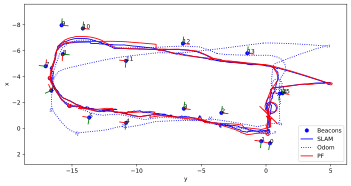
\includegraphics[width=13cm]{PfPath}
\centering
\caption{Particle Filter Path}
\end{figure}

\subsection{Discussion}
The particle filter was able to successfully track the robot without a known starting position. The random resampling worked well and reduced the effect of particle deprivation. This approach could be further improved by altering the quantity of random particles injected, based on the sum of the particle weightings. If the weighted sum of the particles is low, injecting more random particles increases the chance of finding the location of the robot. When the weighted sum of the particles is high, the posterior belief becomes less affected by the random particles. Further improving this approach, an adaptive resampling approach could be implemented such as KLD-Sampling. This controls the quantity of the total particles by measuring the particles distribution across the state space using bins. By adaptively changing the particles the computational cost and variance of the estimated likelihood can both be minimized. Another area of improvement is the motion model. While the odometry model provided accurate measurements for the particles to move during periods with no beacons in sight. It could be improved by fusing the model with the command velocities via an estimator such as BLUE. This is useful information that can improve the motion models prediction.  


\section{SLAM}
\begin{figure}[h]
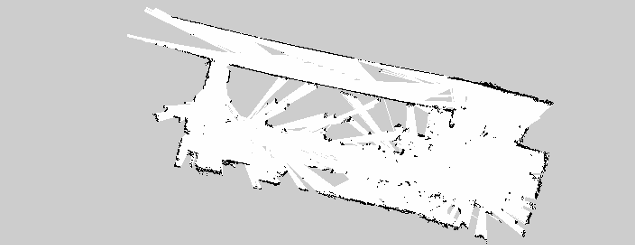
\includegraphics[width=8cm]{slam}
\centering
\caption{Turtlebot SLAM Algorithm}
\end{figure}
if a cell is free (white), unknown (grey) or occupied (black). The map produced has successfully closed the loop, thus the robot has recognised a previous location and updated previous beliefs based on this. The corridor appears slightly bent in the map. This is because the corridor contains little to no features so it must rely on the odometry which drifts over time. Areas of the corridor were left greyed out. This could be because the robot didn’t see this part or was processing previous information, missing the readings. Within the room, there occupied areas scattered. The algorithm failed to identify the area occupied by the desks as they all look the same. 


%\appendix
%\section{Sensor models}

%\comment{Include your calibration plots here.}

\color{blue}
\section*{Instructions}

\begin{enumerate}
\item The reports can be created in Word or \LaTeX.  Use the
  appropriate template but delete all the instructions in blue.  

\item The page limit is five pages with an optional one page appendix.
  No title pages please.  We will deduct 10\% for every page over the
  page limit.  Do not squeeze the margin or use small fonts (12pt
  please).

\item Ensure your names and group number are in the title block.

\item No abstract, introduction, or conclusion is required.
  
\item Submit your reports as a PDF document through Learn.  We will
  deduct 10\% for non PDF documents.

\item Have a read of my guidelines for writing a report,
  \url{https://eng-git.canterbury.ac.nz/mph/report-guidelines/blob/master/report-guidelines.pdf}
  
\end{enumerate}


\end{document}

